\documentclass[11pt,twocolumn]{article}

\usepackage[a4paper,margin=0.75in,columnsep=0.28in]{geometry}
\usepackage{times}
\usepackage{graphicx}
\usepackage{booktabs}
\usepackage{tabularx}
\usepackage{array}
\usepackage{amsmath}
\usepackage{url}
\usepackage{microtype}
\usepackage[font=small,labelfont=bf]{caption}

\graphicspath{{../artifacts_final/}{artifacts_final/}}
\setlength{\parindent}{1em}
\setlength{\parskip}{0.22em}
\setlength{\floatsep}{0.55em}
\setlength{\textfloatsep}{0.65em}
\setlength{\intextsep}{0.55em}

\title{\textbf{Financial Complaint Classification and Shortcut Robustness}}
\author{Maksim Petrenko \and Timur Khairislamov\\
NLP in Python, HSE University}
\date{}

\begin{document}
\maketitle

\begin{abstract}
We study product classification for consumer financial complaints and ask whether strong NLP models learn robust complaint semantics or mainly exploit surface lexical shortcuts. We compare TF-IDF with Logistic Regression, frozen DistilBERT embeddings with Logistic Regression, and fine-tuned DistilBERT. Clean test performance alone suggests that fine-tuned DistilBERT is best, but the margin over TF-IDF is very small: 0.852 versus 0.848 macro-F1. Robustness tests give the more important result. After masking top TF-IDF features, fine-tuned DistilBERT loses 0.387 macro-F1, while TF-IDF loses 0.184. This suggests that transformer fine-tuning does not automatically remove shortcut learning. We therefore add calibration, selective prediction, and retrieval support analysis to make the classifier behavior easier to inspect.
\end{abstract}

\section{Problem and motivation}
Financial complaint triage can be treated as a standard text classification problem: given a complaint narrative, predict the financial product category. However, a useful triage system should do more than maximize held-out accuracy. It should be robust to wording changes, reasonably calibrated, and transparent enough for risky predictions to be reviewed.

This task is especially vulnerable to shortcut learning. Product labels often have obvious lexical markers: \textit{mortgage}, \textit{credit report}, \textit{debt}, \textit{bank account}, and \textit{card}. A model can perform well by recognizing these words without learning much about the broader complaint. Our research question is:

\begin{quote}\small
\textbf{When classifying consumer financial complaints, do classical and transformer-based NLP models learn robust product semantics, or do they mainly exploit lexical shortcuts?}
\end{quote}

We answer this by comparing models not only on clean test data, but also under masking perturbations, calibration checks, confidence-based abstention, retrieval-based evidence, and qualitative error analysis.

\section{Dataset and task}
We use consumer complaint narratives from the Consumer Financial Protection Bureau complaint database. The input is the free-text complaint narrative and the target is the product category. To keep the experiment balanced and reproducible, we use five classes and cap the dataset at 1200 examples per class: Bank account or service, Credit card, Credit reporting, Debt collection, and Mortgage. The final test set contains 900 examples, with 180 examples per class.

\begin{figure}[t]
    \centering
    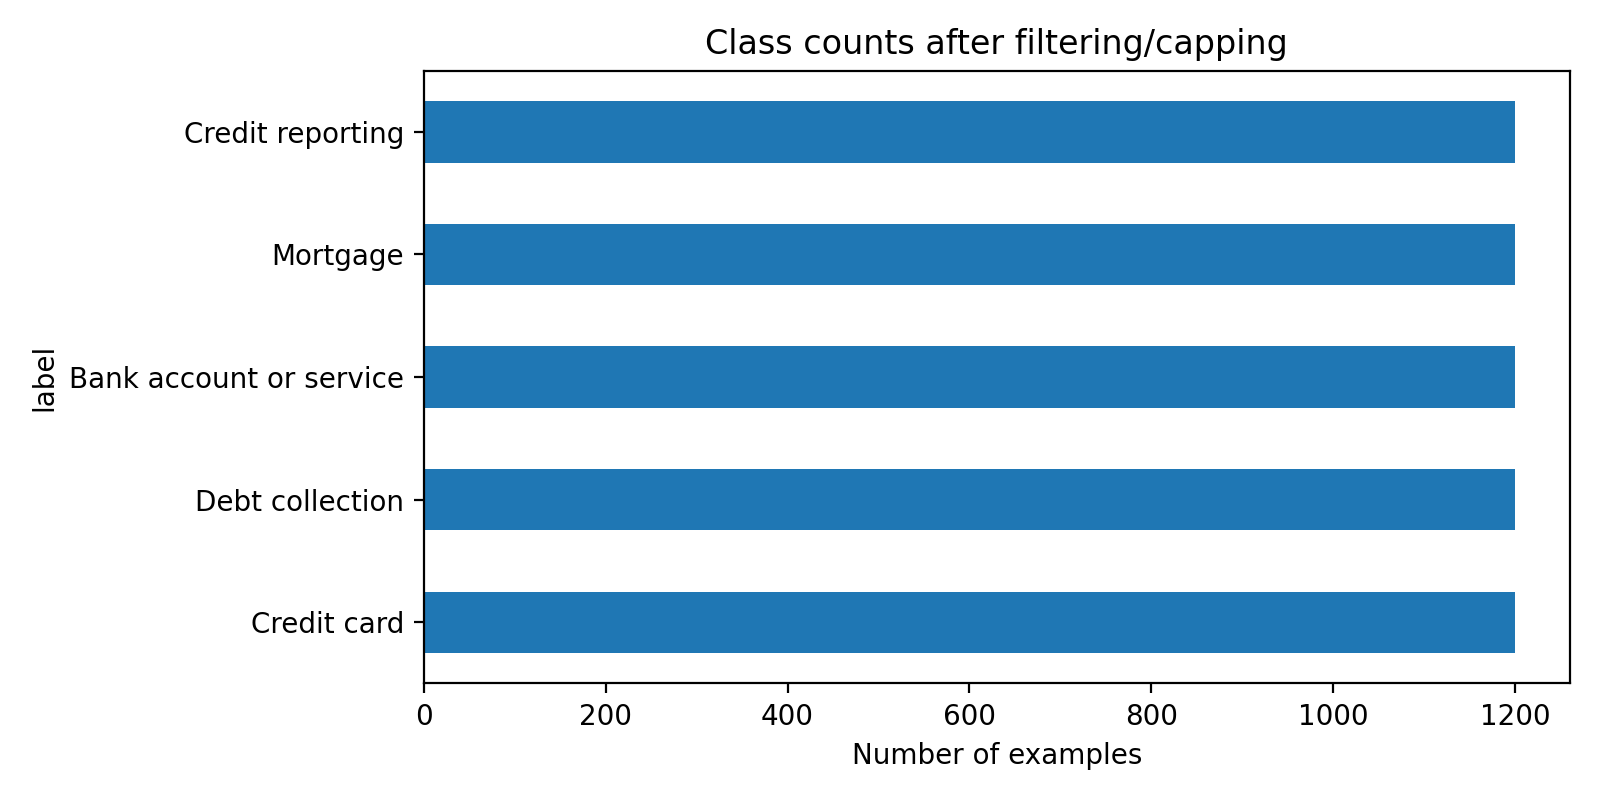
\includegraphics[width=0.92\linewidth]{class_counts.png}
    \caption{Balanced class counts used in the experiment.}
    \label{fig:class-counts}
\end{figure}

The data is split into train, validation, and test sets using stratification. The validation set is used for model selection, while the test set is reserved for the final comparisons.


\begin{table}[t]
\centering
\small
\setlength{\tabcolsep}{3pt}
\begin{tabularx}{\linewidth}{lX}
\toprule
Class & Typical high-weight lexical cues \\
\midrule
Bank account & bank, money, branch, funds, deposit \\
Credit card & card, credit card, balance, capital \\
Credit reporting & experian, equifax, transunion, report \\
Debt collection & debt, collection, calls, collect \\
Mortgage & mortgage, loan, modification, home, escrow \\
\bottomrule
\end{tabularx}
\caption{Examples of TF-IDF Logistic Regression cues. These features are predictive, but they also show why shortcut learning is plausible.}
\label{tab:cues}
\end{table}

\section{Models}
We compare three models with different levels of complexity.

\textbf{TF-IDF + Logistic Regression.} This is the main classical baseline. Texts are represented with word unigrams and bigrams using TF-IDF weighting. A multinomial Logistic Regression classifier is then trained on top. This model is fast, strong, and interpretable through feature coefficients.

\textbf{Frozen DistilBERT embeddings + Logistic Regression.} DistilBERT is used only as a feature extractor. We mean-pool token embeddings and train Logistic Regression on the resulting sentence vectors. This tests whether generic contextual representations are enough without task-specific fine-tuning.

\textbf{Fine-tuned DistilBERT.} The main neural model is \texttt{distilbert-base-uncased} with a classification head. We fine-tune it for three epochs with learning rate $2\cdot10^{-5}$, batch size 16, weight decay 0.01, and maximum sequence length 256. The best checkpoint is selected by validation macro-F1. The notebook saves all generated tables and figures to \texttt{artifacts\_final/}, which makes the report reproducible without manually copying outputs. Random seeds are fixed where possible, and all models use the same train, validation, and test split.

\section{Evaluation protocol}
We use macro-F1 as the main metric because all five classes should matter equally. Accuracy, weighted-F1, and mean confidence are also reported.

To test shortcut reliance, we evaluate each trained model on two modified versions of the test set. In \textbf{product cue masking}, we replace common product terms such as \textit{credit}, \textit{report}, \textit{mortgage}, \textit{loan}, \textit{card}, \textit{bank}, \textit{account}, \textit{debt}, and \textit{collector}. In \textbf{top-feature masking}, we replace the strongest positive TF-IDF Logistic Regression features for each class. The robustness drop is
\[
\Delta = \text{Macro-F1}_{\text{original}} - \text{Macro-F1}_{\text{masked}}.
\]

We also compute Expected Calibration Error (ECE), build selective-prediction curves, and retrieve the five nearest training complaints using TF-IDF cosine similarity. Retrieval support is the fraction of retrieved neighbors whose label agrees with the model prediction.

\section{Clean test results}
Table~\ref{tab:standard} shows the clean test-set comparison. Fine-tuned DistilBERT is the best model, but only by a small margin over TF-IDF: 0.852 versus 0.848 macro-F1. This means the task is strongly lexicalized and a linear TF-IDF model already captures much of the useful signal. Frozen DistilBERT embeddings perform much worse, which suggests that task-specific fine-tuning is important.

\begin{table}[t]
\centering
\small
\setlength{\tabcolsep}{3pt}
\begin{tabular}{lccc}
\toprule
Model & Acc. & Macro-F1 & Conf. \\
\midrule
TF-IDF + LR & 0.848 & 0.848 & 0.761 \\
Frozen BERT + LR & 0.724 & 0.726 & 0.932 \\
Fine-tuned BERT & \textbf{0.852} & \textbf{0.852} & 0.895 \\
\bottomrule
\end{tabular}
\caption{Clean test-set performance. The transformer is best, but the gain over TF-IDF is very small.}
\label{tab:standard}
\end{table}

The two strongest models also make many errors on the same examples. Out of 900 test complaints, both are correct on 721 examples and both are wrong on 91. Fine-tuned DistilBERT fixes 46 TF-IDF mistakes, while TF-IDF fixes 42 DistilBERT mistakes. This again suggests that the final conclusion should not be simply ``BERT beats TF-IDF''. The confusion matrices in Figures~\ref{fig:cm-tfidf} and~\ref{fig:cm-bert} show that both strong models still confuse classes whose narratives naturally mention overlapping financial products.


\begin{figure}[t]
    \centering
    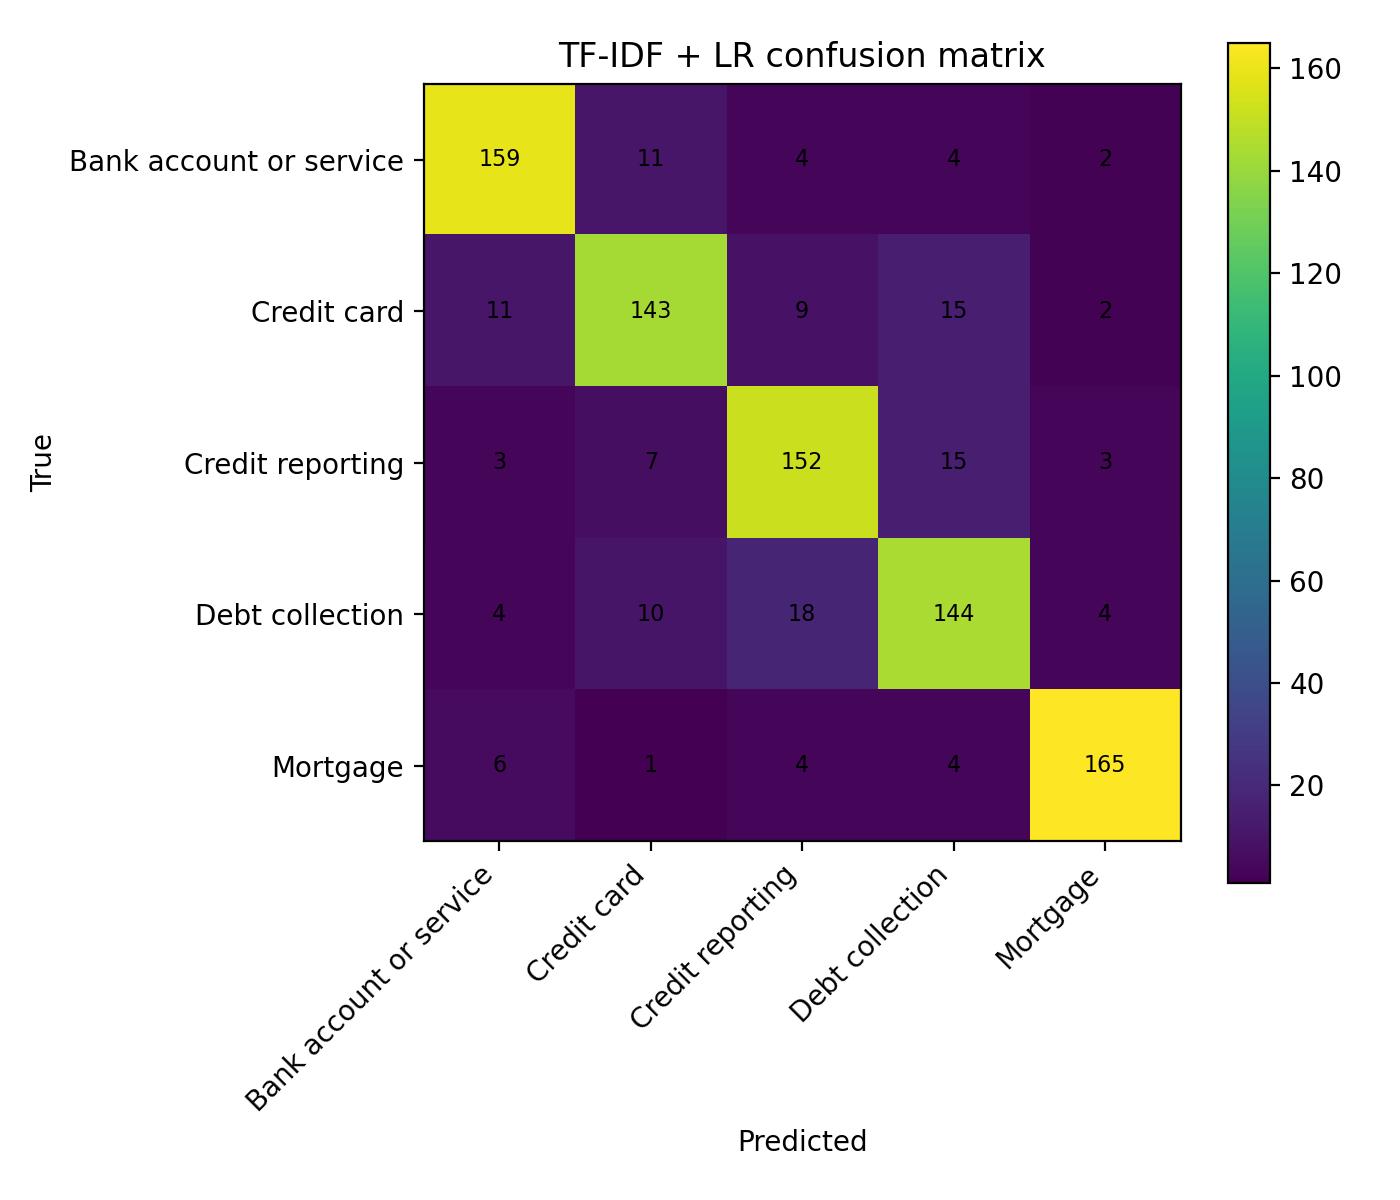
\includegraphics[width=0.88\linewidth]{confusion_tfidf_lr.png}
    \caption{Confusion matrix for TF-IDF + Logistic Regression.}
    \label{fig:cm-tfidf}
\end{figure}

\begin{figure}[t]
    \centering
    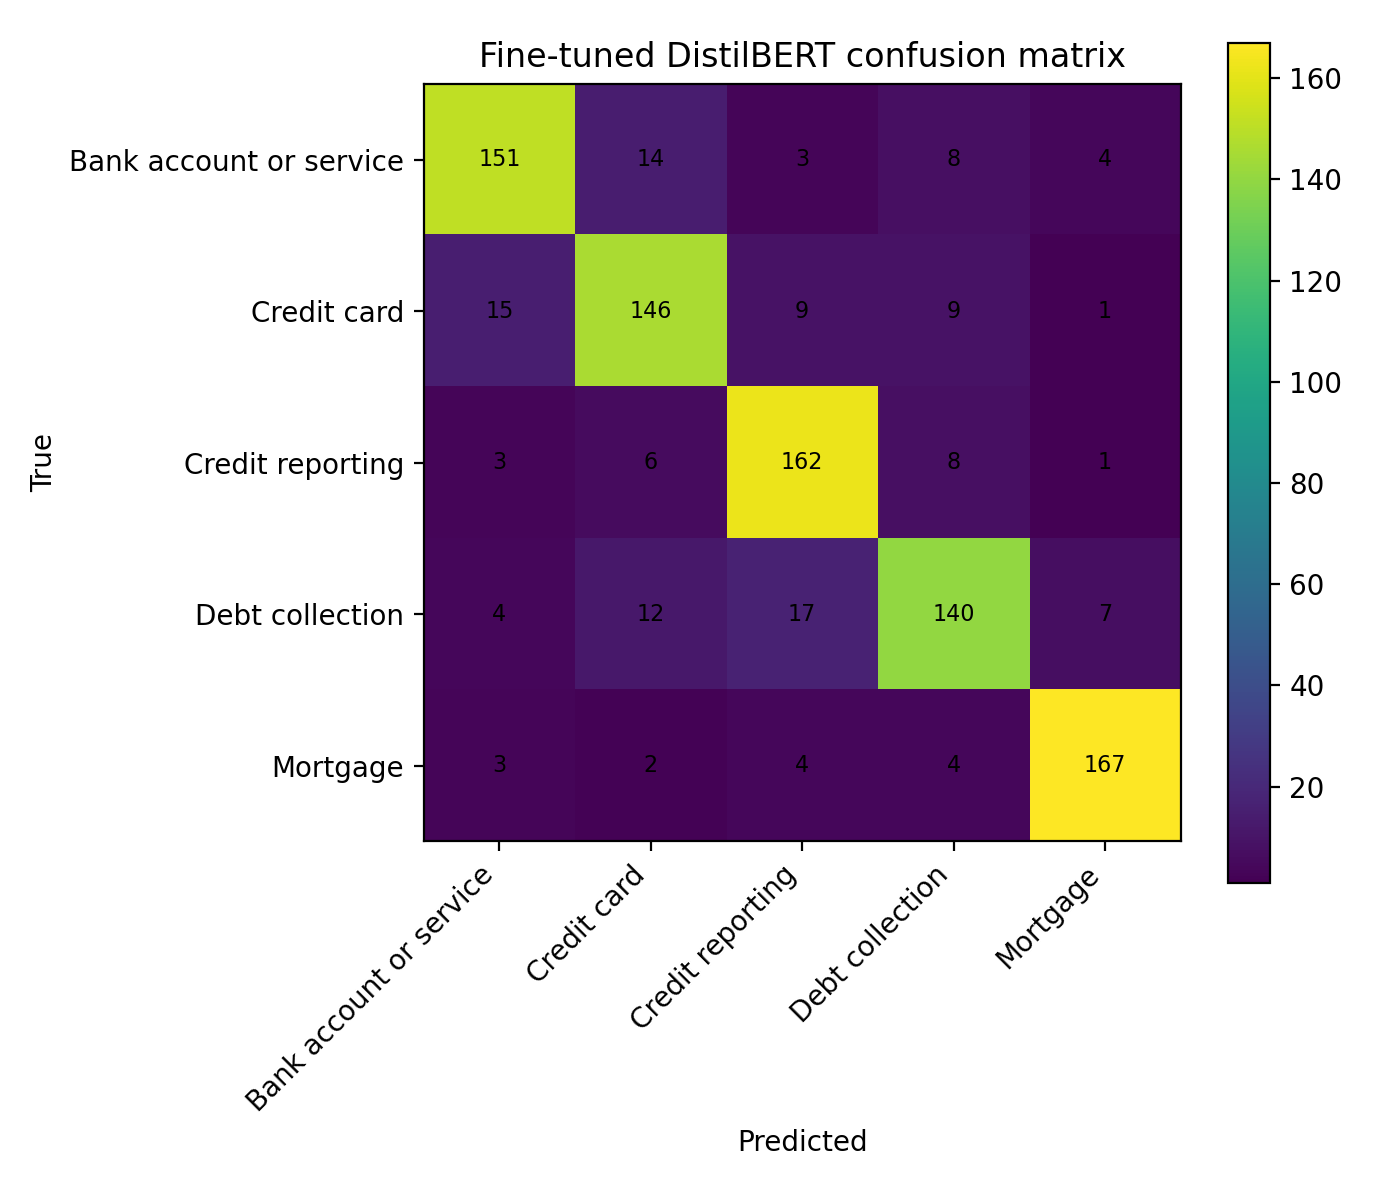
\includegraphics[width=0.88\linewidth]{confusion_finetuned_distilbert.png}
    \caption{Confusion matrix for fine-tuned DistilBERT.}
    \label{fig:cm-bert}
\end{figure}

\section{Shortcut robustness}
The robustness tests are the central part of the project. Table~\ref{tab:robustness} shows that fine-tuned DistilBERT is much more fragile under lexical masking than TF-IDF. Under product cue masking, TF-IDF drops by 0.068 macro-F1, while fine-tuned DistilBERT drops by 0.133. Under top-feature masking, TF-IDF drops by 0.184, while fine-tuned DistilBERT drops by 0.387.

\begin{table}[t]
\centering
\small
\setlength{\tabcolsep}{3pt}
\begin{tabular}{lccc}
\toprule
Model & Original & Cue mask & Top mask \\
\midrule
TF-IDF + LR & 0.848 & \textbf{0.780} & \textbf{0.664} \\
Frozen BERT + LR & 0.726 & 0.576 & 0.257 \\
Fine-tuned BERT & \textbf{0.852} & 0.719 & 0.465 \\
\midrule
TF-IDF drop & -- & \textbf{0.068} & \textbf{0.184} \\
Fine-tuned drop & -- & 0.133 & 0.387 \\
\bottomrule
\end{tabular}
\caption{Macro-F1 under masking. Fine-tuned DistilBERT has the best clean score, but it degrades more strongly than TF-IDF.}
\label{tab:robustness}
\end{table}

\begin{figure}[t]
    \centering
    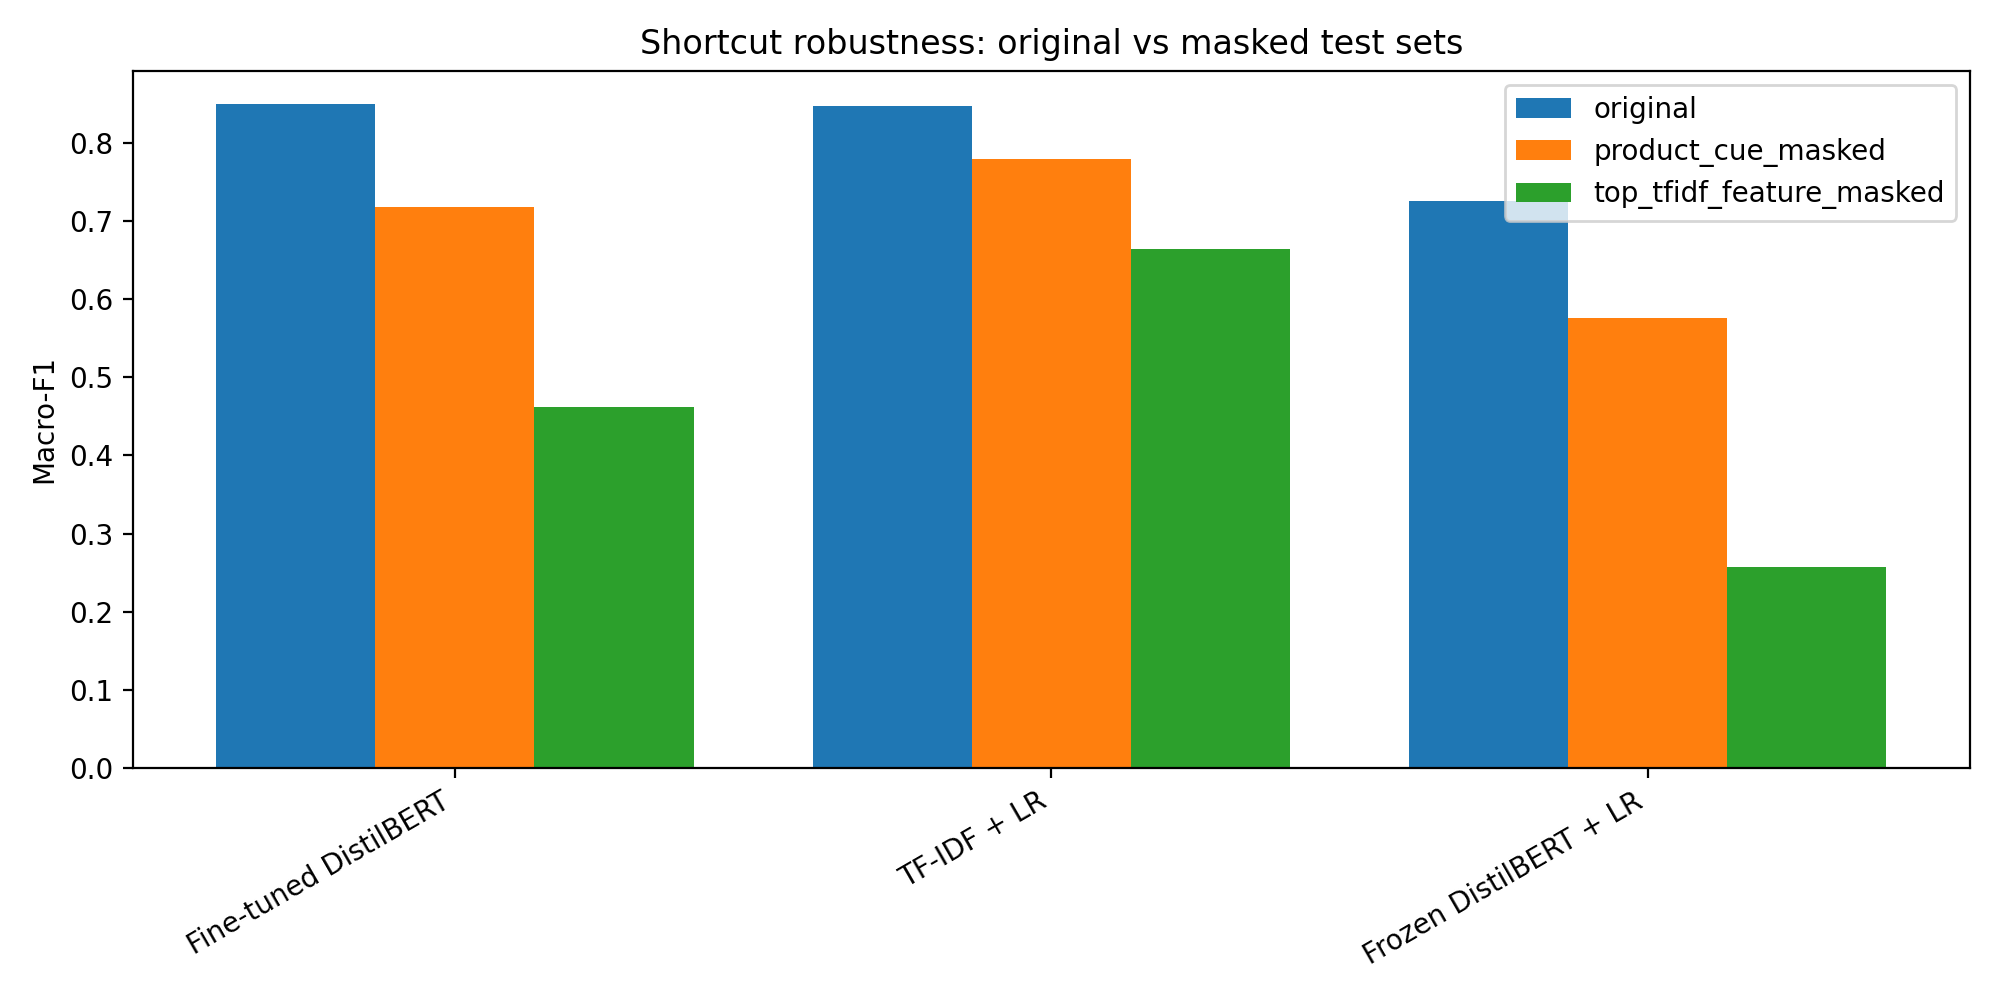
\includegraphics[width=0.96\linewidth]{robustness_macro_f1_bar.png}
    \caption{Macro-F1 on original and masked test sets. The large masked-performance gap is the main evidence for shortcut reliance.}
    \label{fig:robustness}
\end{figure}

This is not what we would expect if the fine-tuned transformer had learned a much deeper semantic representation. A possible explanation is that TF-IDF has many correlated backup features: when one product cue is removed, related n-grams still remain. DistilBERT may be more sensitive because masking key words changes the contextual representation more globally. The masking test is artificial, so it is not perfect causal proof, but it is strong evidence that clean accuracy alone is insufficient.

\section{Calibration and selective prediction}
Calibration is important because a real triage system can route uncertain cases to manual review. Fine-tuned DistilBERT has the best ECE at 0.046. TF-IDF is also reasonable at 0.087. Frozen DistilBERT embeddings are problematic: despite only 0.724 accuracy, their mean confidence is 0.932, giving ECE 0.207.

\begin{table}[t]
\centering
\small
\setlength{\tabcolsep}{3pt}
\begin{tabular}{lccc}
\toprule
Model & ECE & Conf. & Acc. \\
\midrule
TF-IDF + LR & 0.087 & 0.761 & 0.848 \\
Frozen BERT + LR & 0.207 & 0.932 & 0.724 \\
Fine-tuned BERT & \textbf{0.046} & 0.895 & \textbf{0.852} \\
\bottomrule
\end{tabular}
\caption{Calibration summary. Lower ECE is better.}
\label{tab:calibration}
\end{table}

Selective prediction works well for the two strong models. Around 80\% coverage, fine-tuned DistilBERT reaches 0.923 accuracy and TF-IDF reaches 0.918. Around 60\% coverage, fine-tuned DistilBERT reaches 0.967 accuracy and TF-IDF reaches 0.950. This suggests that confidence thresholding is useful when manual review is available.

\begin{figure}[t]
    \centering
    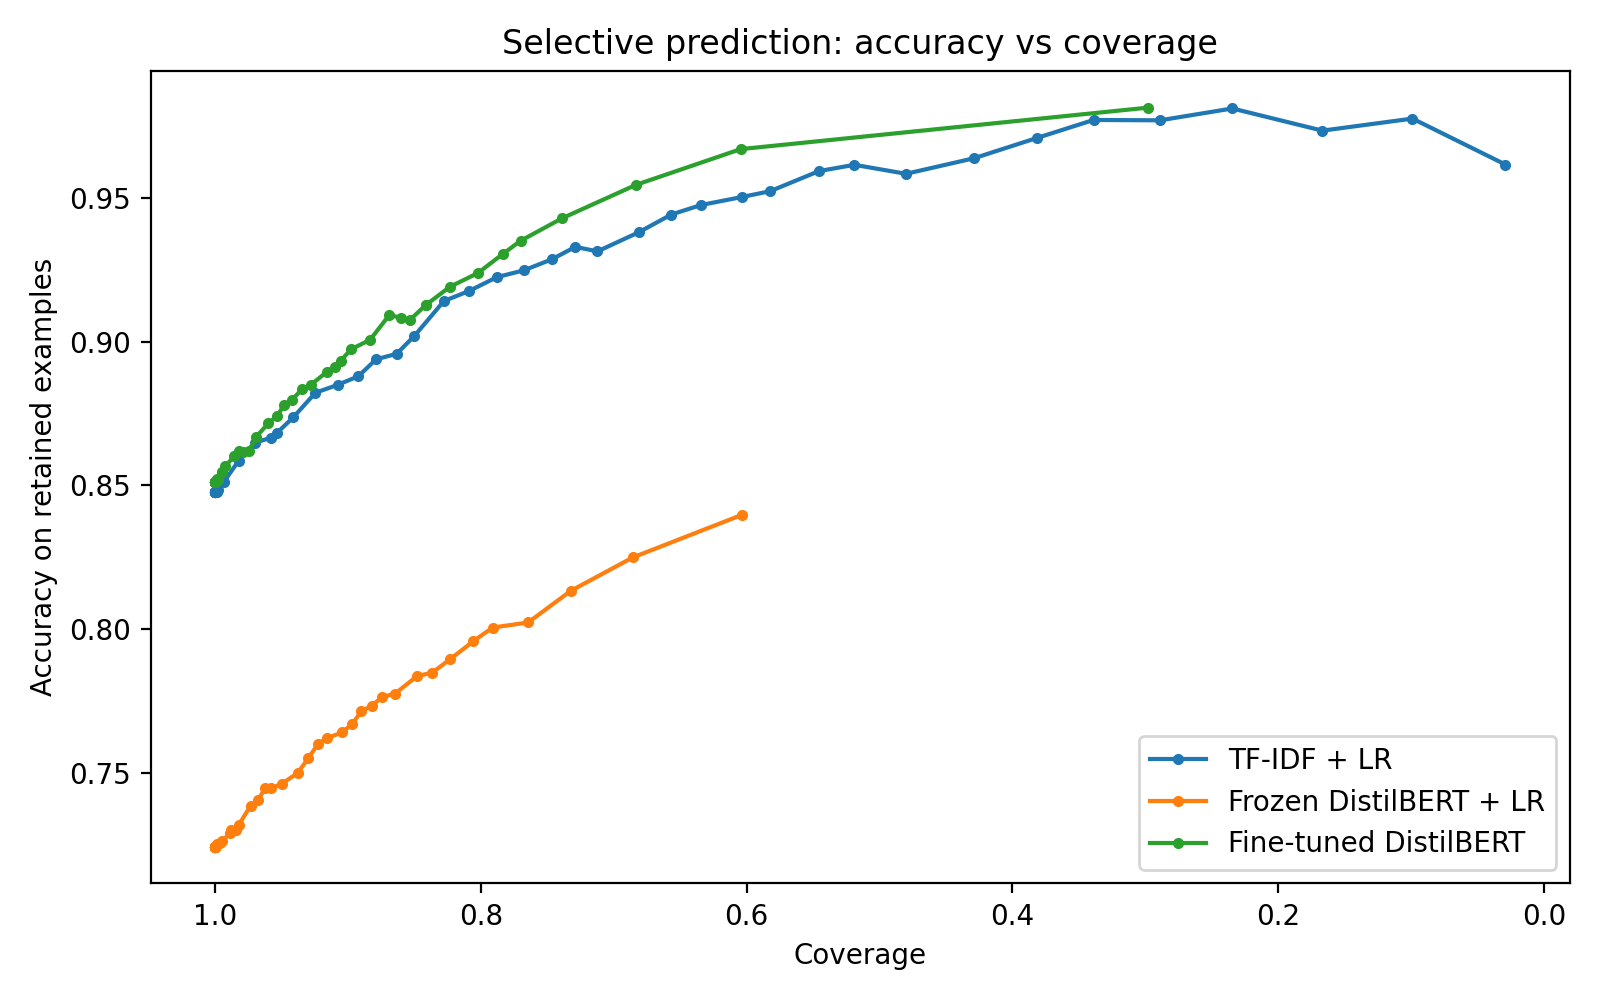
\includegraphics[width=0.96\linewidth]{selective_accuracy_vs_coverage.png}
    \caption{Selective prediction: rejecting low-confidence examples increases accuracy on retained examples.}
    \label{fig:selective}
\end{figure}

\section{Retrieval support and errors}
Predictions are easier to inspect when we can retrieve similar training complaints. For each test example, we retrieve five nearest neighbors and measure whether their labels support the model prediction.

Retrieval support is strongly related to correctness. For fine-tuned DistilBERT, examples with very low support have 0.351 accuracy, while examples with very high support have 0.974 accuracy. The same pattern appears for TF-IDF: 0.395 accuracy at low support and 0.964 at high support. This makes retrieval support useful for flagging risky predictions.

\begin{figure}[t]
    \centering
    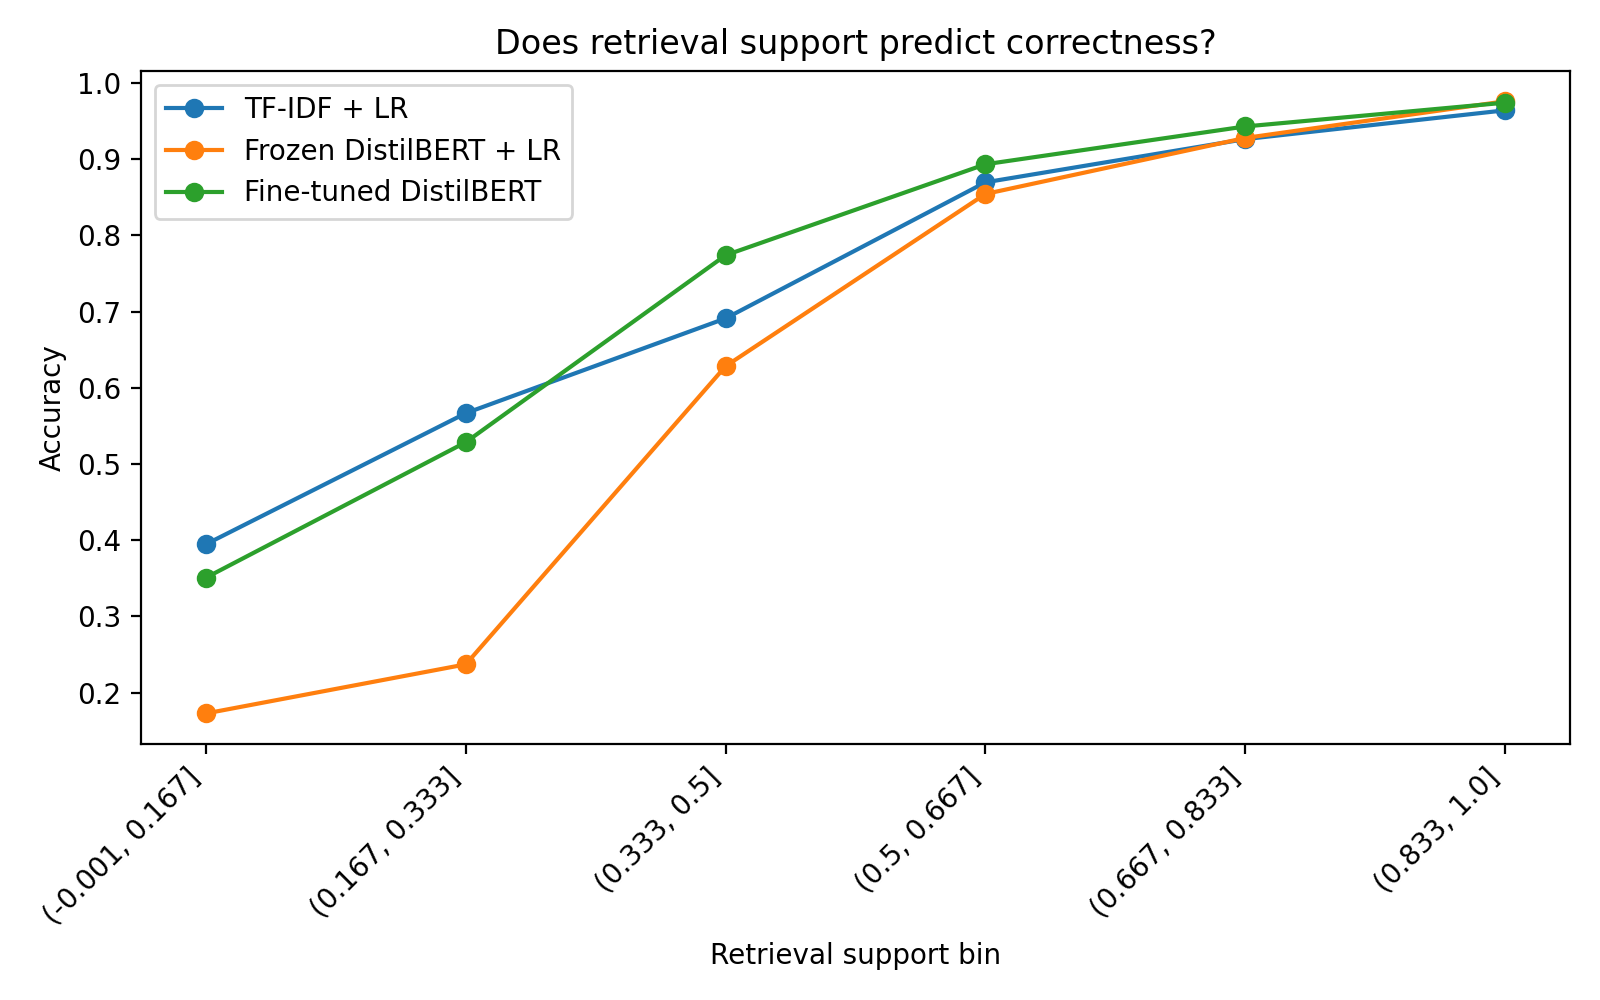
\includegraphics[width=0.96\linewidth]{retrieval_support_vs_accuracy.png}
    \caption{Accuracy increases as retrieved neighbors increasingly agree with the model prediction.}
    \label{fig:retrieval}
\end{figure}

Qualitative errors are often genuinely ambiguous. A single narrative can mention a bank account, credit card, debt collector, and credit report together. DistilBERT sometimes helps when the broader context resolves such conflicts, but it also makes high-confidence mistakes. This supports the final system view: the classifier should be paired with confidence thresholds and retrieval evidence.

\section{Discussion and limitations}
The main lesson is not that transformer models are useless. Fine-tuned DistilBERT is the best clean-test model and the best calibrated model. However, the gain over TF-IDF is tiny, and the transformer is more fragile under our masking tests. Strong classical baselines are therefore essential: without TF-IDF, the transformer result would look more impressive than it actually is.

The main limitation is that masking creates artificial text. Replacing important words with mask tokens may hurt transformer models more than linear models because the input distribution changes. Also, the dataset is balanced for controlled comparison, while real complaint distributions are not balanced. Finally, retrieval is based on TF-IDF similarity; a semantic retriever could be tested in future work. Another limitation is that we do not claim the selected five classes cover the whole complaint taxonomy. They are enough for a controlled robustness study, but a deployed system would need to handle more products and distribution shift over time.

\section{Conclusion}
This project shows that financial complaint classification is highly lexicalized. Fine-tuned DistilBERT reaches the best clean macro-F1, but TF-IDF is almost tied. Under shortcut masking, fine-tuned DistilBERT degrades much more strongly than TF-IDF. Therefore, transformer fine-tuning does not automatically solve shortcut learning.

A practical complaint-triage pipeline should not rely only on one predicted label. It should combine a strong classifier with robustness checks, calibrated confidence, selective prediction, and retrieval-based evidence. This gives a more honest view of when the model is likely to be reliable and when the example should be reviewed manually.

\begin{thebibliography}{9}\small
\bibitem{devlin2019bert}
Jacob Devlin, Ming-Wei Chang, Kenton Lee, and Kristina Toutanova. 2019. BERT: Pre-training of Deep Bidirectional Transformers for Language Understanding. In \textit{NAACL-HLT}.

\bibitem{sanh2019distilbert}
Victor Sanh, Lysandre Debut, Julien Chaumond, and Thomas Wolf. 2019. DistilBERT, a distilled version of BERT: smaller, faster, cheaper and lighter. arXiv:1910.01108.

\bibitem{cfpb}
Consumer Financial Protection Bureau. Consumer Complaint Database. \url{https://www.consumerfinance.gov/data-research/consumer-complaints/}
\end{thebibliography}

\end{document}
